{\color{blue}
\section{Framework Resources Quantification Model}\label{model}

\begin{figure*}
    \centering
	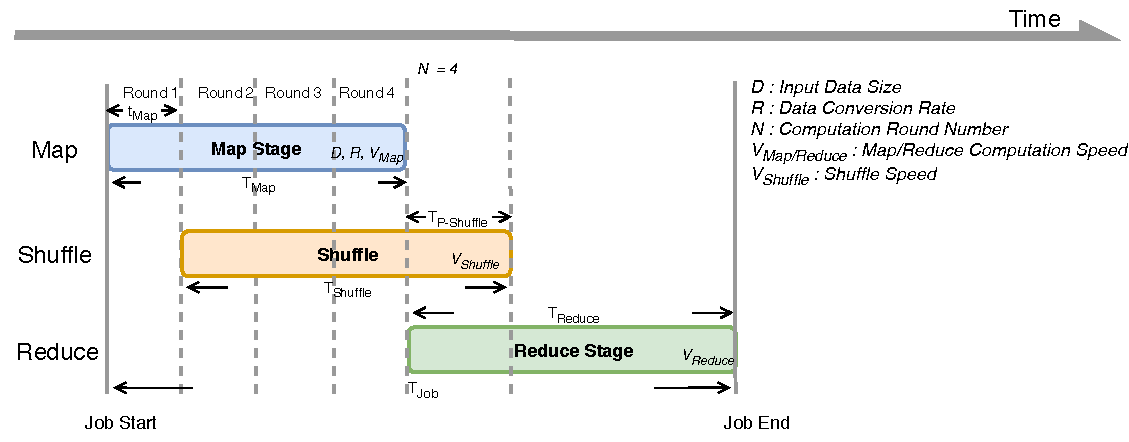
\includegraphics[width=0.85\textwidth]{fig/model_basic}
	\caption{\color{blue}FRQ Model}
    \label{fig:model_basic}
    \vspace{-1em}
\end{figure*}

In this chapter, we introduce \textit{Framework Resources Quantification}(FRQ) model to describe the performance of DAG frameworks.
FRQ model quantifies computing and I/O resources and displays them in time dimension. According to FRQ model, we can calculate the execution time required by the application under any circumstances, including different DAG framework, hardware environment, and so on. Therefore FRQ model is able to help us analyze the resources scheduling of DAG framework and evaluate their performance. We will first introduce FRQ model in Subsection \ref{model_overview}. In the following Subsection \ref{model_analysis}, we will use FRQ model to describe three different computation job and analyze their performance. In the last Subsection \ref{model_verification}, we will use the actual experimental results to verify the FRQ model.

\subsection{The FRQ Model}\label{model_overview}
The current distributed parallel computing frameworks mostly use \textit{Directed acyclic graphs}(DAGs) to describe computation logic. A shuffle phase is required between each adjacent DAG computation phase. In order to better analyze the relationship between the computation phase and the shuffle phase, we propose FRQ model. After quantifying computing and I/O resources, FRQ model is able to describe different resource scheduling strategies. For convenience, we introduce FRQ model by taking a simple MapReduce as an example in this section.

Figure \ref{fig:model_basic} shows how the FRQ model describes a MapReduce task. FRQ model has five input parameters:
\begin{enumerate}
	\item Input Data Size\((D)\): The data size of the computation phase.
	\item Data Conversion Rate\((R)\): The conversion rate of the input data to the shuffle data during a computation phase. This conversion rate depends on the algorithm used in the computation phase.
    \item Computation Round Number\((N)\): The number of rounds needed to complete the computation phase using the current computation resources. The number of rounds depends on the current computation resources and the settings of the computation job. Take Hadoop MapReduce as an example, suppose we have 50 CPUs and enough memory, the Map phase consists of 200 map tasks. Then we need 4 rounds of computation to complete the Map phase.
    \item Computation Speed\((V_{i})\): 
    The computation speed for each computation phase. The computation speed depends on the algorithm used in the computation phase.
    \item Shuffle Speed\((V_{Shuffle})\): 
    Transmission speed during shuffle. Shuffle speed depends on Network and storage device bandwidth.
\end{enumerate}

We can calculate the execution time of each phase of the job with these five parameters. Obviously, the total execution time of job in this case is the sum of the Map phase time and Reduce phase time:
\begin{equation}
\label{equation_Tjob}
\begin{aligned}
    T_{Job} &= T_{Map} + T_{Reduce}
\end{aligned}
\end{equation}
Map phase time depends on input data size and Map computation speed:
\begin{equation}
\label{equation_Tmap}
\begin{aligned}
    T_{Map} &= {{\frac{D}{V_{Map}}}}
\end{aligned}
\end{equation}
The Reduce phase time formula is as follows:
\begin{equation}
\label{equation_Treduce}
\begin{aligned}
    T_{Reduce} &= \frac{D \times R}{V_{Reduce}} + K \times T_{P\_Shuffle}
\end{aligned}
\end{equation}
\(\frac{D \times R}{V_{Reduce}}\) represents the ideal computation time, and \(K \times T_{P\_Shuffle}\) represents the calculated overhead. \(K\) is empirical value.The overhead depends on the parallel time of shuffle phase and the Reduce phase.The parallel time is denoted by \(T_{P\_Shuffle}\). And the total time of shuffle phase is represented by \(T_{Shuffle}\). Because the computatinon of the Reduce phase relies on the data transfer results of the Shuffle phase, a portion of the computation in the Reduce phase need to wait for the transfer results. The overhead is caused by these waiting. The FRQ model uses K to indicate the extent of the waiting.

\begin{equation}
\label{equation_Tshuffle}
\begin{aligned}
    T_{Shuffle} &= {{\frac{D}{V_{Shuffle}}}}
\end{aligned}
\end{equation}

For shuffle-heavy computing jobs, we can optimize the job completion time by reducing \(T_{P\_Shuffle}\). Improving IO speed is a effective way to reduce shuffle time. Another optimization method is to use the idle IO resources in the Map phase for pre-fetching(see Figure \ref{fig:model_basic}). Both of the above methods can effectively reduce \(T_{P\_Shuffle}\). When using FRQ model to describe a computation job, we can easily analyze the resource scheduling strategy of the computation framework. Different computing frameworks may use different resource scheduling strategies. FRQ model can evaluate the scheduling strategies of these computing frameworks and help us optimize them.

\subsection{Model Analysis}\label{model_analysis}

\begin{figure}
	\centering
	\begin{minipage}[hb]{\linewidth}
		\begin{subfigure}{\linewidth}
			\begin{minipage}{\linewidth}
				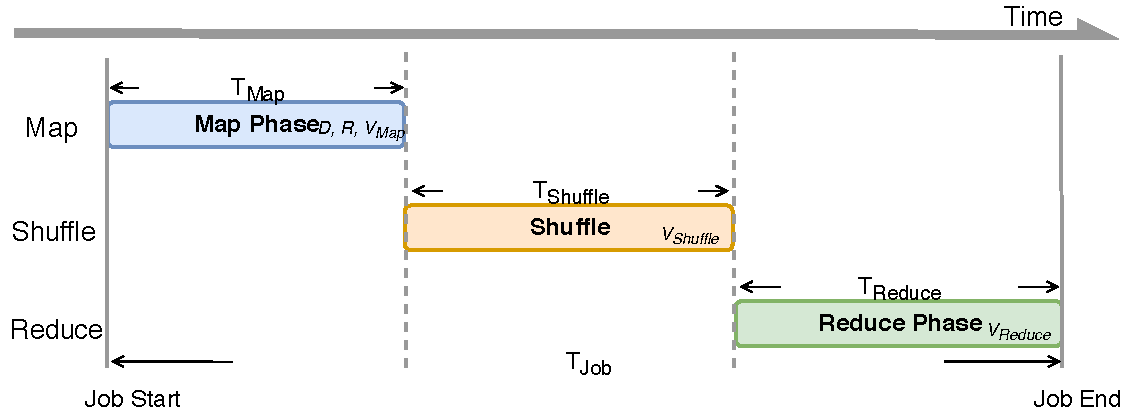
\includegraphics[width=\linewidth]{fig/model_original}
				\caption{\color{blue}Full Serial Mapreduce}
				\label{fig:model_original}
			\end{minipage}
			\begin{minipage}{\linewidth}
				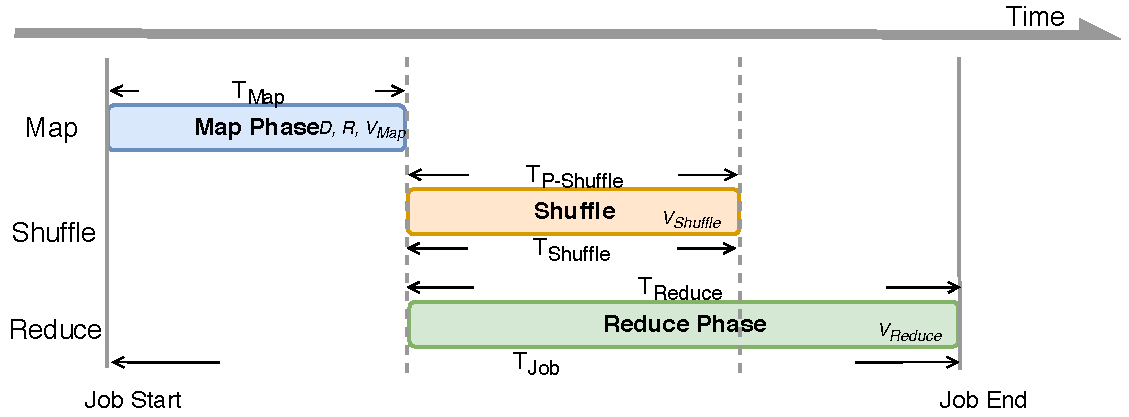
\includegraphics[width=\linewidth]{fig/model_hadoop}
				\caption{\color{blue}Hadoop Mapreduce}
				\label{fig:model_hadoop}
			\end{minipage}
		\end{subfigure}
		\caption{\color{blue}FRQ Model With Different Scheduling Strategies}
		\label{fig:model_strategies}
	\end{minipage}
\end{figure}

FRQ model can describe a variety of resource scheduling strategies. First, we analyze a naive scheduling strategy. As shown in Figure \ref{fig:model_original}, FRQ model describes a Mapreduce job that is fully serially executed. The parallel time of shuffle phase and the Reduce phase is \(0\), in which case \(T_{P\_Shuffle}\) is \(0\). Therefore, the overhead of the Reduce phase is 0. But since shuffle and computation are serial execution, the total execution time of job becomes longer:
\begin{equation}
\label{equation_Tjob2}
\begin{aligned}
    T_{Job} &= T_{Map} + T_{Shuffle} + T_{Reduce}
\end{aligned}
\end{equation}
Obviously, this is an inefficient scheduling strategy. No computing framework uses this scheduling method. Due to serialization, the IO resource is idle during the Reduce phase and Map phase. The scheduling strategy is naive and has a lot of room for optimization.

Figure \ref{fig:model_hadoop} shows the scheduling strategy of Hadoop Mapreduce. In Hadoop Mapreduce, Shuffle phase and Reduce phase start at the same time. In this case, \(T_{P\_Shuffle}\) is equal to \(T_{Shuffle}\). Due to the increase in \(T_{P\_Shuffle}\), the time of Reduce phase will increase(see equation \ref{equation_Treduce}). Because the Shuffle phase and the computation phase are executed in parallel, the total execution time of job is the sum of \(T_{Map}\) and \(T_{Reduce}\)(see equation \ref{equation_Tjob}). The execution time of Shuffle phase is hidden in the Reduce phase. This scheduling strategy is much more efficient than the one in Figure 1. However, after analyzing this model, we found that the IO resource in the Map phase is idle. This scheduling strategy can be optimized.

\begin{figure}
	\centering
	\begin{minipage}[hb]{\linewidth}
		\begin{subfigure}{\linewidth}
			\begin{minipage}{\linewidth}
				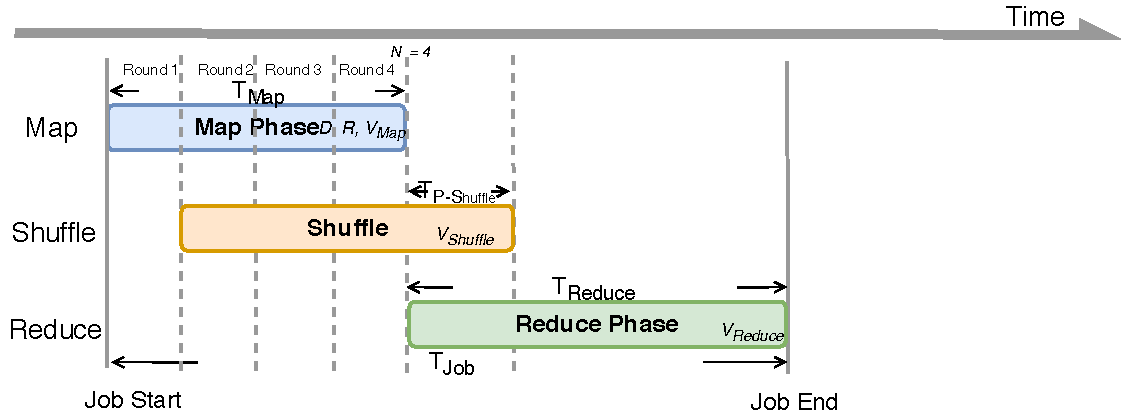
\includegraphics[width=\linewidth]{fig/model_scache1}
				\caption{\color{blue}If \(V_{Map} \times R \ge V_{Shuffle}\)}
				\label{fig:model_scache1}
			\end{minipage}
			\begin{minipage}{\linewidth}
				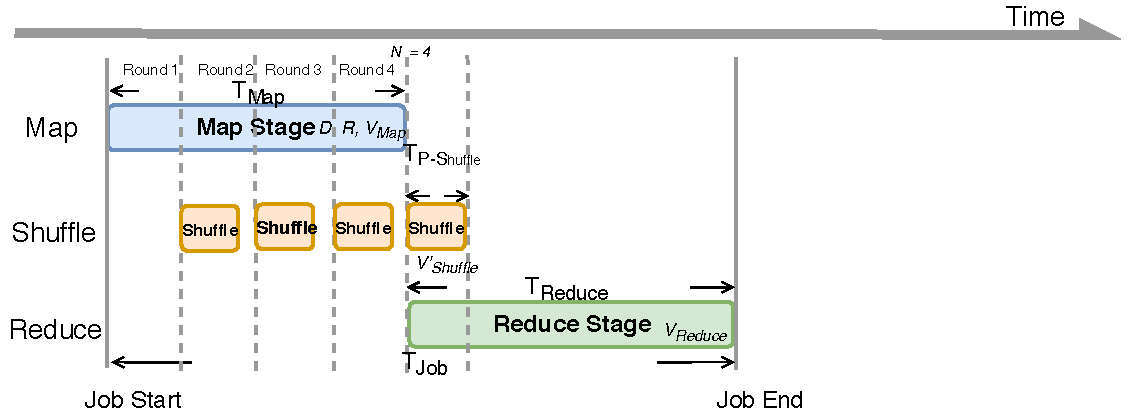
\includegraphics[width=\linewidth]{fig/model_scache2}
				\caption{\color{blue}If \(V_{Map} \times R < V_{Shuffle}\)}
				\label{fig:model_scache2}
			\end{minipage}
		\end{subfigure}
		\caption{\color{blue}FRQ Model With SCache}
		\label{fig:model_scache}
	\end{minipage}
\end{figure}

Figure \ref{fig:model_scache} shows the scheduling strategy for Hadoop Mapreduce with SCache (Suppose N is 4). SCache starts pre-fetching and pre-scheduling in the Map phase. This scheduling strategy can make better use of resources and avoid IO resources being idle in the Map phase. According to the design of SCache pre-fetching, we found that using FRQ model to describe the scheduling strategy of SCache needs to distinguish two situations:

\begin{itemize}
    \item 
    \(V_{Map} \times R \ge V_{Shuffle}\)(Figure \ref{fig:model_scache1}): 
	The meaning of \(V_{Map} \times R\) is the speed at which shuffle data is generated. The meaning of the inequality is that the speed of generating shuffle data(\(V_{Map} \times R\)) is greater than or equal to the shuffle speed(\(V_{Shuffle}\)). When the Round1 of the Map phase ends, the SCache starts shuffling data until the end of the shuffle phase. Due to shuffle speed is slower, the shuffle phase is uninterrupted. SCache transmit the shuffle data generated in the last round of Map phase during the Reduce phase. Therefore \(T_{PShuffle}\) is equal to one-\(N\) of the total time of the shuffle phase:
	\begin{equation}
		\label{equation_Tpshuffle1}
		\begin{aligned}
			T_{P\_Shuffle} &= T_{Shuffle} - \frac{(N - 1)\times T_{Map}}{N}
		\end{aligned}
	\end{equation}
	
    \item \(V_{Map} \times R < V_{Shuffle}\)(Figure \ref{fig:model_scache2}): 
	When the speed of generating shuffle data(\(V_{Map} \times R\)) is less than the shuffle speed(\(V_{Shuffle}\)), SCache needs to wait for shuffle data to be generated. As Figure \ref{fig:model_scache2} shown, the shuffle phase will be interrupted in each Round. Thus \(T_{P_Shuffle}\) is equal to the total time of shuffle (\(T_{Shuffle}\)) minus the time that shuffle is executed in the Map phase:
	\begin{equation}
		\label{equation_Tpshuffle2}
		\begin{aligned}
			T_{P\_Shuffle} &= T_{Shuffle} \times \frac{1}{N}
		\end{aligned}
	\end{equation}
\end{itemize}

% After analyzing the above two situations, we figure out the formula for \(T_{P\_Shuffle}\):
% \begin{equation}
%     \label{equation_Tpshuffle}
%     \begin{aligned}
%     T_{P\_Shuffle} &=
%         \begin{cases} 
%         T_{Shuffle} - \frac{(N - 1)\times T_{Map}}{N} & , V_{Map} \times R \ge V_{Shuffle} \\ 
%         T_{Shuffle} \times \frac{1}{N} & , V_{Map} \times R < V_{Shuffle}
%         \end{cases}
%     \end{aligned}
% \end{equation}
% If the shuffle speed is slow(\(V_{Map} \times R \ge V_{Shuffle}\)), SCache transmit the shuffle data generated in the last round of Map phase during the Reduce phase. Therefore \(T_{PShuffle}\) is equal to one-\(N\) of the total time of the shuffle phase.

% If the shuffle speed is fast (\(V_{Map} \times R < V_{Shuffle}\)), \(T_{P_Shuffle}\) is equal to the total time of shuffle (\(T_{Shuffle}\)) minus the time that shuffle is executed in the Map phase.

Compared to the original Hadoop Mapreduce resource scheduling strategy, Hadoop Mapreduce with SCache reduces \(T_{P\_Shuffle}\) and thus lessens \textit{Reduce Time}(\(T_{Reduce}\)). This is how pre-fetching optimizes the total execution time of job.


\begin{table*}[!t]
\renewcommand{\arraystretch}{1.3}
\caption{\color{blue}Hadoop Mapreduce on 4 nodes cluster in FRQ model}
\label{table1}
\centering
\(D\): GB, \(V_{i}\): GB/s, \(T_{i}\): s
\begin{tabular}{|c||c|c|c|c|c|c|c||c|c|c|c|c|c|c|}
\hline
 &
\(D\) &	
\(R\) &	
\(N\) &	
\(V_{Map}\) &	
\(V_{Reduce}\) &	
\(V_{Shuffle}\) &	
\(K\) &	
\(T_{Map}\) &	
\(T_{Shuffle}\) &	
\(T_{P\_Shuffle}\) &
\(T_{Reduce}\) & 
\(T_{Job}\) & 
\(Exp T_{Job}\) &
\(Error\)\\

\hline
 & 16	& 1	& 2 &	0.65 &	1 &	0.47 &	0.5 &	24.62 &		34.04	 &	21.73 &	26.87 &	51.48	& 55  &		6.39\% \\
 SCache
 & 32	& 1	& 4 &	0.65 &	1 &	0.47 &	0.5 &	49.23 &		68.09	 &	31.16 &	47.58 &	96.81	& 104 & 	6.91\% \\
 & 48	& 1	& 6 &	0.65 &	1 &	0.47 &	0.5 &	73.85 &		102.13 &	40.59 &	68.29 &	142.14	& 151 & 	5.87\% \\
 & 64	& 1	& 8 &	0.65 &	1 &	0.47 &	0.5 &	98.46 &		136.17 &	50.02 &	89.01 &	187.47	& 193 & 	2.87\% \\
 \hline
 & 16	& 1 & 2 &	0.65 &	1 &	0.47 &	0.6 &	24.62 &		34.04	&	34.04	&	36.43	&	61.04	&	73	&	16.38\%	\\
 Legacy
 & 32	& 1 & 4 &	0.65 &	1 &	0.47 &	0.6 &	49.23 &		68.09	&	68.09	&	72.85	&	122.08	&	135	&	9.57\%	\\
 & 48	& 1 & 6 &	0.65 &	1 &	0.47 &	0.6 &	73.85 &		102.13	&	102.13	&	109.28	&	183.12	&	188	&	2.59\%	\\
 & 64	& 1 & 8 &	0.65 &	1 &	0.47 &	0.6 &	98.46 &		136.17	&	136.17	&	145.70	&	244.16	&	249	&	1.94\%	\\
\hline
\end{tabular}
\end{table*}
% \subsection{Performance Analysis}\label{model_performance_analysis}

\begin{table*}[!t]

\renewcommand{\arraystretch}{1.3}
\caption{\color{blue}Hadoop Mapreduce on 50 AWS m4.xlarge nodes cluster in FRQ model}
\label{table2}
\centering
\(D\): GB, \(V_{i}\): GB/s, \(T_{i}\): s
\begin{tabular}{|c||c|c|c|c|c|c|c||c|c|c|c|c|c|c|}
\hline
 &
\(D\) &	
\(R\) &	
\(N\) &	
\(V_{Map}\) &	
\(V_{Reduce}\) &	
\(V_{Shuffle}\) &	
\(K\) &	
\(T_{Map}\) &	
\(T_{Shuffle}\) &	
\(T_{P\_Shuffle}\) &
\(T_{Reduce}\) & 
\(T_{Job}\) & 
\(Exp T_{Job}\) &
\(Error\)\\

\hline
& 128	& 1 & 5 &	1.15 &	1.46	&	1.4 &	0.5 &	111.30 &	91.43	&	18.29	&	96.81	&	208.12	&	232	&	10.29\%	\\
SCache
& 256	& 1 & 5 &	1.15 &	1.46	&	1.4 &	0.5 &	222.61 &	182.86	&	36.57	&	193.63	&	416.24	&	432	&	3.65\%	\\
& 384	& 1 & 5 &	1.15 &	1.46	&	1.4 &	0.5 &	333.91 &	274.29	&	54.86	&	290.44	&	624.36	&	685 &	8.85\%	\\
% & 512	& 1 & 5 &	1.15 &	1.46	&	1.4 &	0.5 &	445.22 &	365.71	&	91.43	&			&	841.62	&	1135 &	25.85\%	\\
\hline
& 128	& 1 & 5 &	1.15 &	1.46	&	1.4 &	0.6 &	111.30 &	91.43	&	91.43	&	142.53	&	253.83	&	266 &	4.57\%	\\
Legacy
& 256	& 1 & 5 &	1.15 &	1.46	&	1.4 &	0.6 &	222.61 &	182.86	&	182.86	&	285.06	&	507.67	&	524 &	3.12\%	\\
& 384	& 1 & 5 &	1.15 &	1.46	&	1.4 &	0.6 &	333.91 &	274.29	&	274.29	&	427.59	&	761.50	&	776 &	1.87\%	\\
% & 512	& 1 & 5 &	1.15 &	1.46	&	1.4 &	0.6 &	445.22 &	365.71	&	365.71	&	588.40	&	1033.62	&	1312 &	21.22\%	\\

\hline
\end{tabular}
\end{table*}

\subsection{Model Verification}\label{model_verification}
In order to verify FRQ model, we run experiment on two environments. The first environment is on Amazon EC2 and it has 50 m4.xlarge nodes as shown in Section \ref{stepup}. Another environment is in our lab. Out lab environment has 4 nodes and each nodes has 128GB and 32 CPUs. To simplify the calculation of the FRQ model, we use Hadoop Mapreduce as framwork(only three phases: \textit{Map, Shuffle,} and \textit{Reduce}) and Terasort as experimental application. We deploye Hadoop with SCache and without SCache on both environments.

Table \ref{table1} shows the calculational results of FRQ model in the lab environment. Workload is from 16 GB to 64 GB. \(D\) and \(N\) are set according to the application parameters. \(R, V_{Map}, V_{Shuffle},\)and \(V_{Reduce}\) are calculated based on experimental results. K is the empirical value, we set \(K\) to 0.5 and 0.6, which reflects that \(T_{P\_Shuffle}\) has less impact on the Reduce phase in the case of SCache. The formulas of \(T_{Job}, T_{Map}, T_{Reduce}\) and \(T_{Shuffle}\) are Equation \ref{equation_Tjob}, Equation \ref{equation_Tmap}, Equation \ref{equation_Treduce} and Equation \ref{equation_Tshuffle}, respectively. In the case of SCache, Terasort on Hadoop Mapreduce satisfies the situation in Figure \ref{fig:model_scache1}(\(V_{Map} \times R \ge V_{Shuffle}\)), thus the formula of \(T_{P\_Shuffle}\) is Equation \ref{equation_Tpshuffle1}. In the case of Legacy, since pre-fetching is not used, \(T_{P\_Shuffle}\) is equal to \(T_{Shuffle}\)(see Equation \ref{equation_Tshuffle}). \(ExpT_{Job}\) represents the actual experiment data, we calculate \(Error\) according to \(T_{Job}\) and \(ExpT_{Job}\). The formular of \(Error\) is:
\begin{equation}
	\label{equation_error}
	\begin{aligned}
		Error &= \frac{ExpT_{Job} - T_{Job}}{T_{Job}}
	\end{aligned}
\end{equation}

Table \ref{table2} shows the calculational results of FRQ model in Amazon EC2 environment. \(V_{Map}, V_{Shuffle},\) and \(V_{Reduce}\) are modified because of the different hardware devices. We also set K to the same empirical value. The formulas in the table are all the same except \(T_{P\_Shuffle}\). In this environment, Terasort on Hadoop Mapreduce satisfies the situation in Figure \ref{fig:model_scache2}(\(V_{Map} \times R < V_{Shuffle}\)), thus the formula of \(T_{P\_Shuffle}\) is Equation \ref{equation_Tpshuffle2}. In the previous case, \(T_{P\_Shuffle}\) is still euqal to \(T_{Shuffle}\).

\begin{figure}
	\centering
	\begin{minipage}[hb]{\linewidth}
		\begin{subfigure}{\linewidth}
			\begin{minipage}{\linewidth}
				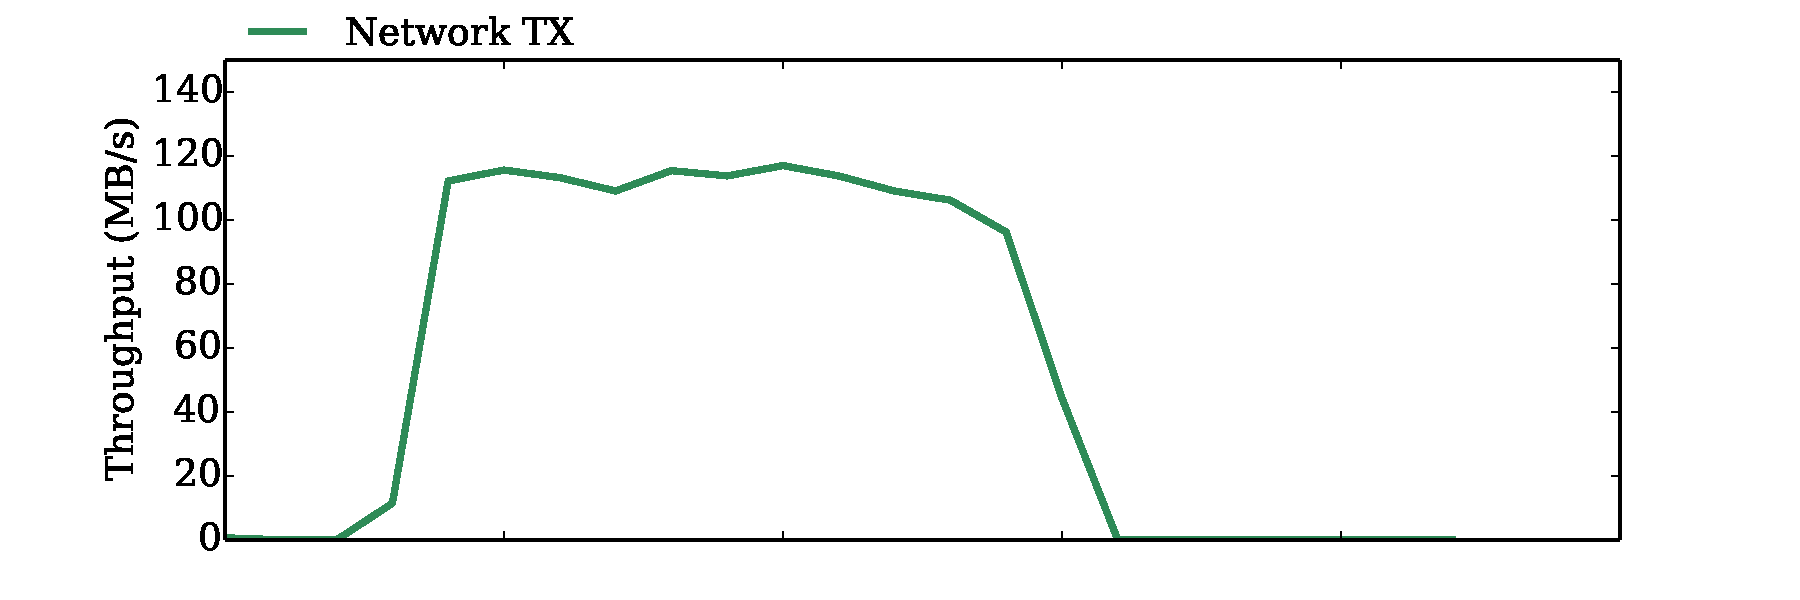
\includegraphics[width=\linewidth]{fig/hadoop_net1}
				\caption{\color{blue}If \(V_{Map} \times R \ge V_{Shuffle}\)}
				\label{fig:hadoop_net1}
			\end{minipage}
			\begin{minipage}{\linewidth}
				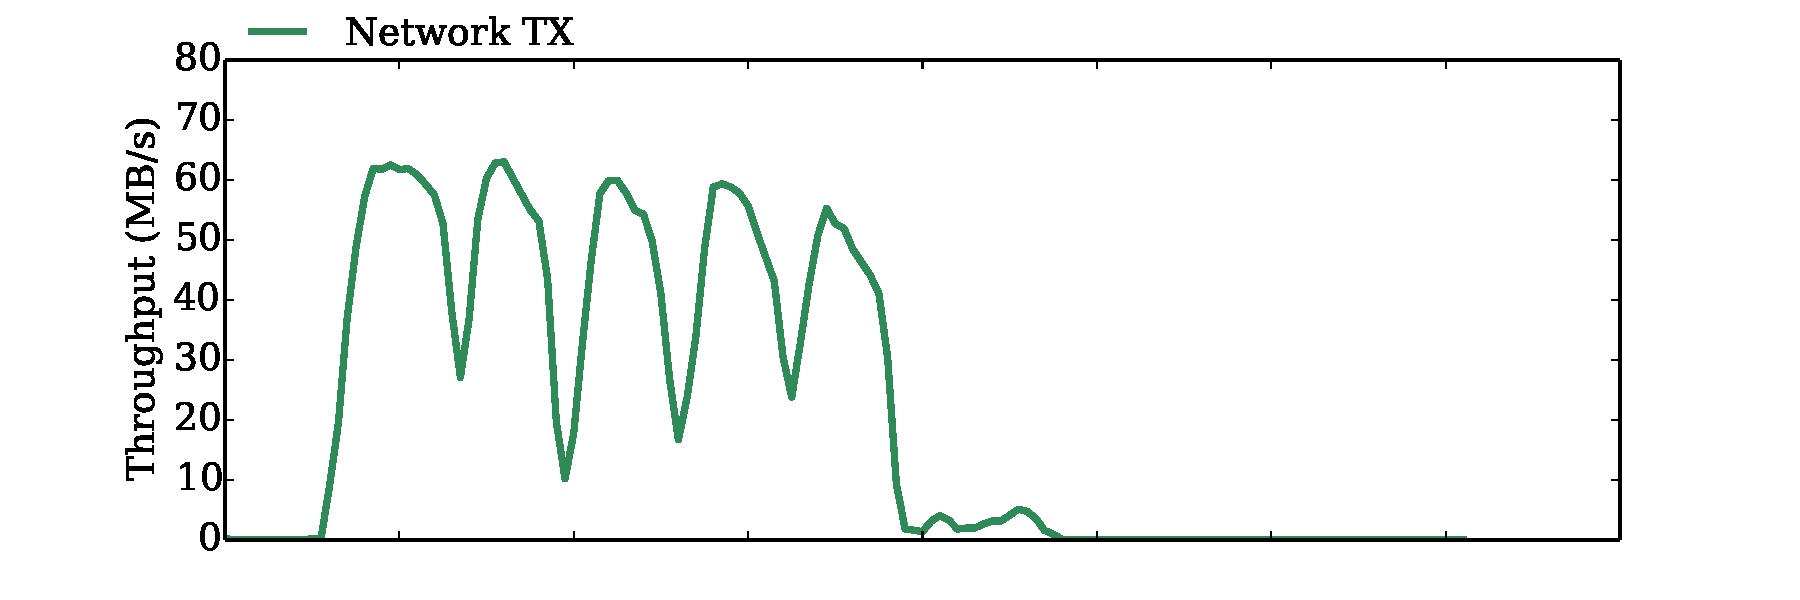
\includegraphics[width=\linewidth]{fig/hadoop_net2}
				\caption{\color{blue}If \(V_{Map} \times R < V_{Shuffle}\)}
				\label{fig:hadoop_net2}
			\end{minipage}
		\end{subfigure}
		\caption{\color{blue}Network utilization on Hadoop Mapreduce with SCache}
		\label{fig:hadoop_net}
	\end{minipage}
\end{figure}

In order to verify the above-mentioned two cases when using SCache, we monitor network utilization and plot it in Figure \ref{fig:hadoop_net}. Figure \ref{fig:hadoop_net1} shows the utilization of Terasort in the lab environment. The network utilization remains high until shuffle phase is complete. This situation is consistent with Figure \ref{fig:model_scache1}. Figure \ref{fig:hadoop_net2} shows the utilization in Amazon EC2 environment. The network utilization is 5 regular peaks, this situation is also consistent with Figure \ref{fig:model_scache2}. Therefore, we believe that FRQ model is able to accurately describe framework with SCache.

In terms of accuracy, the experimental values are all greater than the calculated values. This is because the application has some extra overhead at runtime, such as network warm-up, the overhead of allocating slots, and so on. In the case where the input data is small and the total time is short, the error caused by the overhead is amplified. Overall, the error between \(T_{Job}\) and \(ExpT_{Job}\) is basically below 10\%, such errors are within tolerance . Therefore, We believe that FRQ model can accurately describe DAG framework.
}